\documentclass{article}

\usepackage{ctex}
\usepackage{amssymb}
\usepackage{amsmath}

\usepackage{geometry}
\geometry{a4paper,left=3.18cm,right=3.18cm,top=2.54cm,bottom=2.54cm}

\makeatletter
\newcommand\dlmu[2][4cm]{\hskip1pt\underline{\hb@xt@ #1{\hss#2\hss}}\hskip3pt}
\makeatother

\usepackage{tikz}
\usetikzlibrary{positioning, shapes.geometric}

\usepackage{graphicx}

\begin{document}

\begin{titlepage}
    \centering
    \vspace*{16pt}
    \songti \zihao{1} 哈尔滨工程大学  \\
    \vspace*{36pt}
    \songti \zihao{1} 本科毕业设计(论文)中期进展报告  \\
    \songti \zihao{1} (2021届)  \\
    \vspace*{68pt}
    \songti \zihao{-2} 题目:空间辐射场三维重构方法 \\
    \vspace*{128pt}
    \songti \zihao{3} 学\hspace{1cm}院:\dlmu[5cm]{核科学与技术学院}  \\
    \vspace*{12pt}
    \songti \zihao{3} 专\hspace{1cm}业:\dlmu[5cm]{核工程与核技术}  \\
    \vspace*{12pt}
    \songti \zihao{3} 班\hspace{1cm}级:\dlmu[5cm]{20171516班}  \\
    \vspace*{12pt}
    \songti \zihao{3} 学生姓名:\dlmu[5cm]{刘铭}    \\
    \vspace*{12pt}
    \songti \zihao{3} 学\hspace{1cm}号:\dlmu[5cm]{2017151613}    \\
    \vspace*{12pt}
    \songti \zihao{3} 指导教师:\dlmu[5cm]{宋玉收}  \\
    \vspace*{12pt}
    % \songti \zihao{3} 日\hspace{1cm}期:\dlmu[5cm]{2021年4月8日}    \\
    \vspace*{28pt}
    \lishu \zihao{-2} 哈尔滨工程大学本科生院制
    \thispagestyle{empty}
\end{titlepage}

\section{目前毕业设计(论文)工作进展及取得的成果}
\subsection{调研所得}
\songti\zihao{-4}
空间辐射场三维重构方法是辐射场可视化仿真技术的一项重要技术。辐射场可视化仿真技术不仅能够应用在核设施退役工程,将辐射场的分布以可视化的形式显示在虚拟场景中,评估施工人员所接受的辐射剂量;还能在核与辐射安全科普工作中发挥积极的作用,将辐射场的剂量值、分布等定量信息展现给公众,易于科普工作者与公众进行互动沟通,提高公众对核科学的认识。

对于复杂的辐射场,目前常用的重构方法有两种:“正演”方法和“反演”方法。“正演”方法是通过对辐射传输方程进行求解,在了解放射源基本信息的基础上,构造准确的系统模型进行粒子运输模拟,从而将空间辐射场进行重构;而“反演”方法是在未知放射源基本信息的情况下,通过实际测量获得有限、离散的采样数据进行分析和空间重构,从而获得完整的辐射场分布数据。

“正演”方法目前常用的一些算法有蒙特卡洛法和点核积分法等,其中蒙特卡洛法是通过随机性方法对辐射传输方程进行求解计算,点核积分法是通过确定论方法对辐射传输方程进行求解。当前,国内外对于“正演”方法重构辐射场方法的技术比较成熟,代表性的有美国洛斯阿拉莫斯国家实验室开发的蒙特卡洛辐射输运软件MCNP、欧洲核子研究组织开发的蒙特卡洛应用软件包Geant4、中科院核能安全技术研究所开发的核设计与辐射安全评价软件SuperMC、法国国家能源局开发的用于核辐射工作场所的虚拟现实仿真软件Narveos、比利时核研究中心开发的剂量评估软件VISIPLAN等等。

“反演”方法也指散乱数据重构方法,目前主要有插值和拟合,插值是指已知某函数的在若干离散点上的函数值或者导数信息,通过求解该函数中待定形式的插值函数以及待定系数,使得该函数在给定离散点上满足约束;而拟合是指已知某函数的若干离散函数值,通过调整该函数中若干待定系数,使得该函数与已知点的差别最小。常用的插值算法包括多项式插值、径向基插值、反距离权重插值等,常用的拟合算法包括最小二乘法、最小立方法等。相比于“正演”方法,散乱数据重构方法在辐射场的研究方向仅有少数研究者提出自己的方法。中国工程物理研究院赛雪、韦孟伏提出基于MQ径向基函数散乱插值方法,证明了将MQ径向基插值方法应用于辐射场重构是可行的;华南理工大学王壮、蔡杰进提出网格函数插值法对空间辐射场进行重构,并且提出运用贝叶斯推理对辐射场重构值进行优化。

\subsection{插值算法学习}
\songti\zihao{-4}
1977年,Lee等人提出多层B样条的散乱数据插值方法,首次将样条插值算法拓展到散乱数据领域。凭借样条插值本身相比于高阶多项式插值的优势,样条插值在图像重构、气象时空数据等领域应用得十分广泛。克里金插值算法是由法国科学家乔治马瑟顿提出的一种最优空间插值算法,目前主要应用于地质统计学领域,其算法相比于距离反比加权算法具有更高的计算精度、计算效率以及计算复杂程度。


\subsubsection{样条插值}
\songti\zihao{-4}
样条插值是一种分段多项式,且相邻多项式之间具有一定的连续性。因此,样条函数既具有多项式的使用优点,又保留了各段之间的独立性。

设$ \Omega = \{ (x,y,z) | 0 \leqslant x \leqslant m,0 \leqslant y \leqslant n,0 \leqslant z \leqslant l\} $是$ xyz $空间上的一个立方体区域,在四维空间内有一散乱点集合$ P = \{ ( x,y,z,v ) \} $,其中$ (x,y,z) $是立方体区域内的一点,需要定义一个均匀的三次B样条函数对这些点进行逼近。假设$ \phi $为$ (m+3) \times (n+3) \times (l+3) $的控制点网格。根据控制点确定三次样条函数如下:
\begin{equation}
    f(x,y,z)=\sum_{i=0}^{3}\sum_{j=0}^{3}\sum_{k=0}^{3}B_{i}(r)B_{j}(s)B_{k}(t) \phi_{(a+i)(b+j)(c+k)}
\end{equation}

其中,$ a=[x]-1,b=[y]-1,c=[z]-1,r=x-[x],s=y-[y],t=z-[z]$。$ B_{i}(r)\text{、}B_{j}(s)\text{以及}B_{k}(t) $为均匀三次B样条基函数。

因此,问题转化为求解由控制点集合确定三次B样条函数,如图\ref{三维B样条控制点网格}所示,若要对空间中某一点进行插值,可根据其周围64个控制点的值,求解该区域的样条函数,从而得到该点的预测值。
\begin{figure}
    \centering
    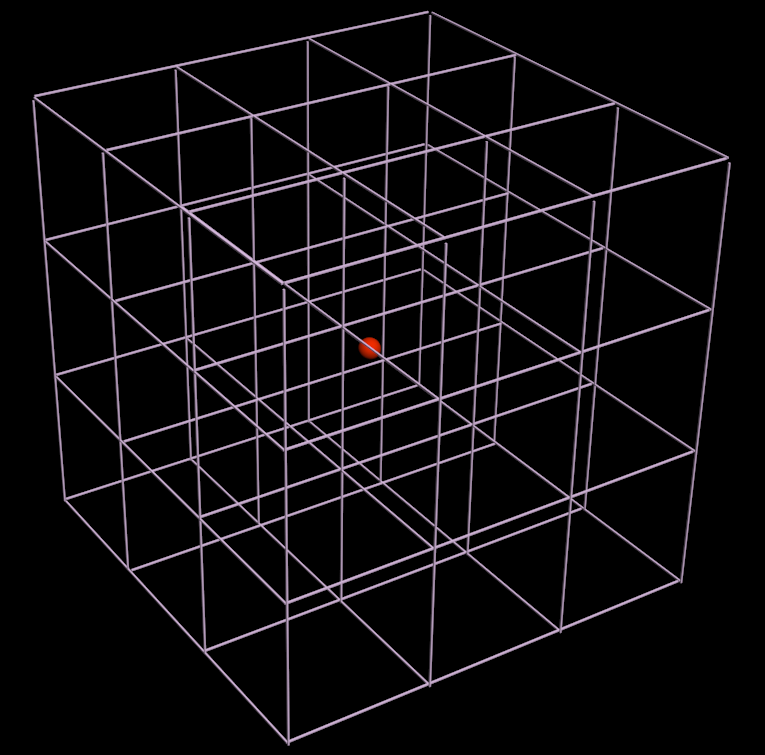
\includegraphics[width=0.7\textwidth]{B-splines.png}
    \caption{三维B样条控制点网格}
    \label{三维B样条控制点网格}
\end{figure}

\subsubsection{克里金插值}
\songti\zihao{-4}
讲述克里金插值之前,先要引入反距离权重插值法的概念。反距离权重插值法的假设是彼此距离较近的事物要比彼此距离较远的事物更相似,因此任何未测量的未知预测值与预测周围的测量值相关,且每个测量值与预测值的权重关系与反距离的$ p $次幂成正比。即对空间中任意一点$ (x,y,z) $的属性$ v(x,y,z) $,定义反距离权重插值公式预测值为:
\begin{equation}
    \hat{v} = \sum_{i=1}^{n} \frac{1}{d^{p}}v_{i}
\end{equation}

其中$ d $为预测点与测量点之间的欧氏距离。

但是反距离权重插值法有一些不可避免的弊端,例如幂次方$ p $的值不能确定以及用倒数来描述空间的关联程度不够准确。因此,为解决这些弊端,克里金插值法被提出。

相比于反距离权重插值,克里金插值的公式较于抽象:
\begin{equation}
    \hat{v_{o}} = \sum_{i=1}^{n}\lambda_{i}v_{i}
\end{equation}

其中,$ \hat{v_{o}} $是点$ (x_{o},y_{o},z_{o}) $处的预测值,$ \lambda_{i} $是权重系数。

克里金插值与反距离权重插值都是用空间上所有已知点的数据加权求和来预测未知点的值,但克里金插值的权重系数并非距离的倒数,而是能够满足点$ (x_{o},y_{o}) $处预测值$ \hat{v_{o}} $与真实值$ v_{o} $之差最小的一套最优系数,即:
\begin{equation*}
    \min_{\lambda_{i}} Var \left( \hat{v_{o}} - v_{o} \right)
\end{equation*}

同时满足无偏估计的条件:
\begin{equation*}
    E\left( \hat{v_{o}} - v_{o} \right) = 0
\end{equation*}

克里金模型分为普通克里金、简单克里金、泛克里金、指示克里金、概率克里金、析取克里金、协同克里金。若用以下公式简单表示辐射场:
\begin{equation}
    V(x,y,z) = \mu(x,y,z) + \varepsilon(x,y,z)
\end{equation}

其中,$ V(x,y,z) $是辐射场剂量值,可分解为确定趋势$ \mu(x,y,z) $和随机的自相关误差$ \varepsilon(x,y,z) $。无论辐射场的趋势如何,都无法完全确定$\mu(x,y,z)$。因此,需要对误差项$ \varepsilon(x,y,z) $做出一些假设,也就是假设$ \varepsilon(x,y,z) $与$ \varepsilon(x+\triangle x,y+\triangle y,z+\triangle z) $之间的自相关误差不取决于绝对位置,而仅仅取决于两点之间的相对位移$ (\triangle x,\triangle y,\triangle z) $,这对于确保重复性以预测自相关函数很有必要。

了解完自相关函数$ \varepsilon $,再来看趋势函数$ \mu $。若趋势函数是常数,即对于空间中所有的点$ (x,y,z) $,$ \mu(x,y,z) = m $,其中$ m $未知,则这种模型就是普通克里金模型。当然,趋势函数可以是线性函数甚至是多项式函数构成,那么由多项式函数构成的趋势函数并且回归系数未知的模型称为泛克里金模型。而趋势函数无论是常数或者多项式,只要趋势函数的所有参量已知,则这种模型为简单克里金模型。若趋势函数为分段函数,则称为指示克里金模型。根据不同的变换,还有析取克里金模型、协同克里金模型、概率克里金变换等。

\subsection{提出创新思路}
\songti \zihao{-4}
空间插值的确定性方法包含反距离权重法IDW(克里金插值)以及径向基函数插值法RBF(B样条插值)等,但仅仅依靠某种单一的方法难以对辐射场重构的很好。因此提出一种新的重构方法,将两种插值的结果进行对比,对于重构出来的两个不同的辐射场,将重构出来的两个辐射场剂量值相差较大的区域,选点进行再次测量,从而最终得到重构辐射场,相比于依靠某单一插值方法,随机选取同样的测量点进行重构插值得到的辐射场,应该会有更好的效果。

\subsection{重构方法程序}
\subsubsection{程序框图}

\begin{tikzpicture}[node distance=10pt]
    \node[draw, rounded corners]                        (start)   {开始};
    \node[draw, below=of start]                         (step 1)  {导入数据};
    \node[draw, below=of step 1]                        (step 2)  {计算Kriging插值重构辐射场};
    \node[draw, below=of step 2]                        (step 3)  {计算Splines插值重构辐射场};
    \node[draw, below=of step 3]                        (step 4)  {计算两个重构辐射场的偏差};
    \node[draw, diamond, aspect=6, below=of step 4]     (choice)  {偏差值是否大于设定值};
    \node[draw, right=20pt of choice]                   (step x)  {添加测量数据};
    \node[draw, below=20pt of choice]                   (step 5)  {绘制空间辐射场};
    \node[draw, below=of step 5]                        (step 6)  {计算整体偏差};
    \node[draw, rounded corners, below=of step 6]       (end)     {结束};

    \draw[->] (start)  -- (step 1);
    \draw[->] (step 1) -- (step 2);
    \draw[->] (step 2) -- (step 3);
    \draw[->] (step 3) -- (step 4);
    \draw[->] (step 4) -- (choice);
    \draw[->] (choice) -- (step 5);
    \draw[->] (choice) -- node[left]  {否} (step 5);
    \draw[->] (choice) -- node[above] {是}  (step x);
    \draw[->] (step 5) -- (step 6);
    \draw[->] (step x) -- (step x|-step 1) -> (step 1);
    \draw[->] (step 6) -- (end);
\end{tikzpicture}

\subsubsection{完成情况}
\songti \zihao{-4}
对于重构方法程序的编写,现已完成80\%以上的工作,对于主体部分——Kriging插值算法以及Splines插值算法已经实现,在不进行辐射场绘制的情况下,现程序已能实现该框图功能。

\section{存在的问题及拟解决措施}
\songti \zihao{-4}
当前论文工作正有序向前推进,后期可能存在的问题与困难有:
\begin{enumerate}
    \item Geant4运用不熟练,后期使用Geant4获得辐射场数据可能遇到困难;
    \item 实验测量放射源剂量率时,由于存在天然本底以及使用的放射源活度较小,并且探测器本身存在一定大小,测量可能存在较大误差;
    \item 通过创新重构方法得到的辐射场,可能在某些情况下,重构效果不如样条插值方法重构的辐射场或者克里金插值方法重构的辐射场;
\end{enumerate}

\section{下一步工作计划}
\songti \zihao{-4}
对于辐射场数据,后期拟通过以下几种方式获得:
\begin{itemize}
    \item 实验测量
    \item Geant4仿真
    \item 点核积分法
\end{itemize}

按照放射性源的个数划分,辐射场可以分为单放射源情况和多放射源情况;按照空间划分,未知空间可以分为简单空间(空间规则且基本没有屏蔽)和复杂空间(空间不规则且存在屏蔽)。对于单放射源情况的简单空间,可以通过实验测量获得;对于多放射源情况,通过Geant4仿真或者点核积分法获得数据;对于复杂空间辐射场,通过Geant4仿真获得数据。

得到辐射场数据后,通过对比克里金插值重构辐射场数据、B样条插值重构辐射场数据以及两种插值重构优化辐射场数据结果,对于创新重构方法效果。

\section{对毕业设计(论文)能否按期完成情况的评价}
\songti \zihao{-4}
目前论文工作整体进度已经稳步推进,重构方法已经基本完成并且采用了几组高斯模拟数据进行重构,得到了预期效果,遇到的问题都在较小的调节范围内,最终的论文可以按时完成。

\end{document}